%% Copernicus Publications Manuscript Preparation Template for LaTeX Submissions
%% ---------------------------------
%% This template should be used for the following class files: copernicus.cls, copernicus2.cls, copernicus_discussions.cls
%% The class files, the Copernicus LaTeX Manual with detailed explanations regarding the comments
%% and some style files are bundled in the Copernicus Latex Package which can be downloaded from the different journal webpages.
%% For further assistance please contact the Publication Production Office (production@copernicus.org).
%% http://publications.copernicus.org


%% Differing comments regarding the specific class files are highlighted.


%% copernicus.cls
\documentclass[acp]{copernicus}

%% copernicus2.cls
%\documentclass[acp]{copernicus2}

%% copernicus_discussions.cls
%\documentclass[journal abbreviation, hvmath, online]{copernicus_discussions}


\begin{document}


\title{Statistical analysis of a LES shallow cumulus cloud ensemble using a 
cloud tracking algorithm}


\author[1]{Jordan T Dawe}
\author[1]{Philip H Austin}

\affil[1]{Department of Earth and Ocean Sciences, 
        University of British Columbia, 
	6339 Stores Road, 
        Vancouver, BC, 
        V6T 1Z4}

%% The [] brackets identify the author to the corresponding affiliation, 1, 2, 3, etc. should be inserted.



\runningtitle{CLOUD TRACKING}

\runningauthor{Dawe and Austin}

\correspondence{Jordan T Dawe\\ (jdawe@eos.ubc.ca)}



\received{}
\pubdiscuss{} %% only important for two-stage journals
\revised{}
\accepted{}
\published{}

%% These dates will be inserted by the Publication Production Office during the typesetting process.


\firstpage{1}

\maketitle



\begin{abstract}
A technique for the tracking of individual clouds in an large eddy simulation 
model is presented.  We use this technique on a Large Eddy Simulation (LES) of 
a shallow cumulus cloud field based upon the Barbados Oceanographic and 
Meteorological Experiment (BOMEX), to calculate statistics of cloud height, 
lifetime, and other physical properies for individual clouds in the model.  We 
also examine the question of nature versus nurture in shallow cumulus clouds: 
do properties at cloud base determine the upper-level properties of the clouds 
(nature), or are cloud properties determined by the environmental conditions 
they encounter (nurture).  We find that clouds which ascend through an 
environment that has been pre-moistened by previous cloud activity are no more 
likely to reach the inversion than clouds that ascend through a drier 
environment.  Conversely, we find that cloud base moisture and liquid-water 
potential temperature are largely uncorrelated with upper-level cloud 
properties, but that the area of the cloud base influences cloud buoyancy and 
maximum cloud height.  We conclude that cloud properties are primarily 
influenced by cloud base area, and thus nature is more important than nurture 
for shallow cumulus clouds.
\end{abstract}

%% only used for copernicus2.clsu
%\abstract{
% TEXT
% \keywords{TEXT}}

\introduction
%% \introduction[modified heading if necessary]

- Clouds are vital for climate
- hard to parameterize
- Studied via LES
- LES studies traditionally look at bulk cloud properties

- Individual plumes
- Arakawa and Shubert
- Zhao and Austin (
- Heus and Jonkers

- Satellite cloud tracking/cloud identification.

- Better would be an automated system

Here we present a fully automated algorithm for the tracking of individual 
clouds in a LES.  In section 2 we describe the BOMEX LES we analyzed, section 
3 presents the cloud tracking algorithm itself, and section 4 presents an 
overview of the statistics generated by the algorithm.  Then in section 5 we 
use the output generated by the algorithm to address the question of whether 
initial cloud properties or the environment encountered by the cloud is more 
important in determining the course of the cloud's life cycle.  Finally in 
section 6 we discuss our results and conclusions.

%==============================================================================

\section{Model Description}

All LES calculations in this paper were made using the System for Atmospheric 
Modeling \citep[SAM;][]{Khairoutdinov2003}.  SAM is an anelastic LES 

The model was run configured as standard Global Energy and Water Cycle 
Experiment (GEWEX) Cloud System Studies \citep[GCSS;][]{Randall2003} Barbados 
Oceanographic and Meteorological Experiment \citep[BOMEX;][]{Siebesma2003} 
experiment.  BOMEX simulates a trade-wind cumulus cloud field observed over 
ocean near Bermuda

The BOMEX run was performed on a 6.4 km x 6.4 km horizontal x 3.2 km vertical 
domain with 25 meter grid resolution in all directions for 6 hours, and the 
first three hours of simulation were discarded.  Model fields were output every 
minute for the last three hours of the simulation, and th

%==============================================================================

\section{Cloud Tracking}

Dividing a cloud field up into individual clouds at a single moment in time is 
a trivial matter of finding connected cloudy regions.  Tracking the resulting 
clouds from one time step to the next is more problematic, as a cloud is a 
process, not a consistent physical object.  A rising parcel of moist air may 
condense, a parcel of air containing condensate may evaporate, and a cloud 
may merge with another cloud or split into multiple clouds.  To handle all of 
these possible events, we adopt a more complex definition of what constitutes 
a cloud.

\subsection{Cloud Tracking Algorithm}

We begin by defining three cloud regions (Fig. \ref{fig:vertical_section}).  
The first is the cloud ``core", defined following \cite{Siebesma1995} as all 
model points containing condensed liquid water which have positive buoyancy and 
upward velocity.  The second we refer to as the ``condensed" region, defined 
simply as all model points containing condensed liquid water.  Third is the 
cloud ``plume", the region of upward moving air that is associated with the 
cloud.  We define this region following the work of \cite{Couvreaux2010} via a 
numerical tracer that is emitted at the surface and subsequently decays 
exponentially with a one minute time constant.  A point is considered to be in 
the plume if the tracer value of that point is larger than one standard 
deviation above the mean tracer value at the current height.  Additionally, 
the tracer must exceed five precent of the integral of the tracer standard 
deviation from the surface to the current height.  However, unlike 
\citeauthor{Couvreaux2010}, we do not require upper-level plume points to have 
condensed liquid water.  Finally, we force the condensed region to be a subset 
of the plume by setting all condensed points to also be plume points.

Next, we divide the cloud field into ``cloudlets" by assigning core points 
which are nearest-neighbour adjacent to the same cloudlet.  These core 
cloudlets are then expanded into nearest-neighbour connected condensed points 
until all condensed points that are connected to a core are assigned to a 
cloudlet.  Condensed points cannot belong to two cloudlets, so if a cloud 
contains more than one contiguous volume of nearest-neighbour connected core 
points it will be split into seperate cloudlets.  Leftover condensed points are 
then divided into new cloudlets which have no cores.  Once all the condensed 
points have been assigned to cloudlets, this expansion process is repeated for 
the plume points.  This results in three types of cloudlets: ones consisting of 
core points surrounded by condensed points surrounded by plume, ones consisting 
of condensed points surrounded by plume, and ones consisting only of plume 
points.  This process is then repeated for every saved model time step.

These cloudlets are then assigned to individual clouds.  For the first time 
step, we assign cloudlets which have touching condensed surfaces to the same 
cloud.  At subsequent time steps, cloudlets that spatially overlap with a cloud 
at the previous timestep are assumed to be the same cloud.  The cloudlet's 
position is corrected for advection using the mean velocity of the cloudlet's 
condensed points (if condensed points are present in the cloudlet) or plume 
(if they are not), multiplied by the time between model output saves.

Four kinds of overlap are possible: condensed points in the cloudlet may 
overlap condensed points in a previous time step cloud 
(condensed$\rightarrow$condensed); condensed points may overlap previous 
plume points (plume$\rightarrow$condensed); plume may overlap condensed 
points (condensed$\rightarrow$plume); and plume may overlap plume 
(plume$\rightarrow$plume).  Several kinds of overlap may occur 
simultaneously, so we define a heirarchy of connection types and check each in 
turn.  The strongest connection type is condensed$\rightarrow$condensed, 
followed by plume$\rightarrow$condensed, then plume$\rightarrow$plume.  
Condensed$\rightarrow$plume connections are ignored, which prevents 
connections between newly formed cloudlets and leftover plume from a 
dissipating cloud.  Conversely, allowing plume$\rightarrow$condensed 
connections lets us associate newly condensed clouds with plumes rising through 
the sub-cloud layer.  Only the strongest connection type present for a given 
cloudlet is considered: if a cloudlet has condensed$\rightarrow$condensed 
connections, any condensed$\rightarrow$plume or plume$\rightarrow$plume 
connections are ignored, and if there are condensed$\rightarrow$plume 
connections, plume$\rightarrow$plume connections are ignored.  

A cloudlet may connect to more than one cloud, which is used to identify merges 
and splits (Fig. \ref{fig:cloudfinder_instructions}).  Any cloudlet which 
overlaps more than one previous time step cloud is considered to be the result 
of a merge between the two clouds.  In this case the cloudlet is assigned to 
the cloud with the largest overlap, and the other overlapping clouds are 
assumed to have merged with the largest overlap cloud.  Next, clouds that 
connect to more than one cloudlet are considered for splitting.  Splits occur 
only if a cloud contains more than one cloudlet whose plume is in contact with 
the ground, with the largest cloudlet being assigned to the original cloud and 
the smaller sub-clouds becoming new clouds. Cloudlets which are not connected 
to the ground are assigned to the nearest ground-connected cloudlet, measured 
by the distance between the centroids of the cloudlets.  Any cloudlets that do 
not overlap clouds in the previous time step are assumed to be new clouds.  
This process of cloudlet assignment, merging, splitting, and creation is 
repeated for each time step until all cloudlets are assigned to a cloud.
  
Once the cloudlets are all assigned to a cloud, any cloud that has condensed 
points for less than five minutes is flagged.  If any merge or split events 
occured over these clouds' short lifetimes, the cloud is rejoined to the cloud 
it split from or merged into.  This prevents decaying detritus shed from a 
cloud top and clouds which split then immediately re-merge with their parent 
from being counted as discrete cloud objects.  Finally, clouds that have 
condensed liquid water for less than two minutes, and thus are unconnected to 
future or past clouds, are placed into a ``cloud noise" group consisting of a 
mixture of ``mistakes" in the tracking algorithm and short-lived, dynamically 
forced clouds at cloud base. 

\subsection{Cloud Tracking Results}

Applying the cloud tracking algorithm to three hours of BOMEX LES output 
resulted in 3171 tracked clouds.  Of these, 609 (19\%) were created by 
splitting an existing cloud, 2381 (75\%) were unassosciated with previous 
clouds, and 181 (6\%) were present at the start of the output period and thus 
their initiation was not observed.  Conversely, 261 (8\%) of the clouds ended 
their life cycle by merging with another cloud, 2820 (89\%) ended their 
lifecycle by decaying away, and 90 (3\%) were present at the end of the output 
period.  Only 20 clouds both begin by splitting from and end by merging with 
another cloud, indicating that 850 clouds (27\%) are involved in such 
interactions--a sizeable proportion of the field.  The larger number of clouds 
present at the start of the output period (181) than at the end (90) is the 
result of the algorithm maintaining connections between physically separated 
clouds.

Figure \ref{fig:example_cloud} displays horizontally averaged cloud properties 
for the longest-lived cloud in the ensemble.  The cloud's cross-sectional area 
shows large, vertically coherent discontinuities in time due to merge events 
and split events.  However, the majority of the merge and split events that 
occur to this cloud do not significantly alter the cloud area, and none of the 
other horizontally averaged properties display significant discontinuities.  
Most of the cloud maintains upward velocities over 1 m s$^{-1}$ (Fig. 
\ref{fig:example_cloud}b), though short-lived downdrafts are apprent in the 
inversion (above $\approx$ 1.5 km) and at the end of the cloud's life.  Near 
cloud base, the total specific water ($q_t$, units of g kg$^{-1}$, Fig. 
\ref{fig:example_cloud}c), liquid-water potential temperature ($\theta_l$, 
units of K, Fig. \ref{fig:example_cloud}d), and condensed liquid water 
($q_l$, units of g kg$^{-1}$, Fig. \ref{fig:example_cloud}e) are similar to 
the environmental properties near cloudbase but the $q_t$ excess, $\theta_l$ 
deficit, and $q_l$ of the cloud increases with height and indications of 
upward propagating pulses can be seen in these fields.  The cloud buoyancy is 
generally positive below the inversion, with strong pulses of positive buoyancy 
apparent (displayed using virtual potential temperature $\theta_v$, units of 
K, Fig. \ref{fig:example_cloud}f).  Finally, comparing this example cloud with 
the example clouds presented by \citet[][figs. 4 and 5]{Heus2009} shows 
similar magnitudes and patterns in cloud properties.

Core properties (with cloud core defined as cloud points having upward velocity
and positive buoyancy) for the same cloud (Fig. \ref{fig:example_core}) 
display buoyant mass pulses more clearly than the cloud properties.  Cloud core 
occupies roughly 60\% the horizontal cloud area near cloud base, but 
essentially vanishes in the inversion.  Since the cloud properties show 
positive vertical velocity and negative buoyancy in the inversion, the 
dissapearance of the core is due to the rapid increase of environmental 
buoyancy which makes the cloud negatively buoyant.  Cloud core vertical 
velocity increases steadily with height and $q_t$ excess, $\theta_l$ deficit, 
and $q_l$ are all greatest at cloud top.  Core buoyancy is positive by 
definition, and regular buoyant pulses are apparent.

\subsection{Tracked Cloud Statistics}

In this section we will examine the statistics of the cloud population 
generated by the cloud tracking algorithm.  Before calculating these 
statistics, we removed any clouds which begin or end outside the model output
period since we do not have access to their complete life cycles. This removed 
287 clouds from the sample, leaving 2,921.  This filtering will tend to remove 
some of the longest-lived clouds from our sample, biasing the population 
slightly.  However, our results show the cloud population to be overwhelmingly 
composed of short-lived clouds, implying that robust estimates of the frequency 
occurrance of the longest-lived clouds will not be possible in any case.

Both cloud lifetime (Fig \ref{fig:cloud_stats}a) and mean cloud area over the 
cloud's lifetime (Fig \ref{fig:cloud_stats}b) are heavily skewed toward small, 
short-lived clouds.  Over 1,000 of the tracked clouds, a little less than a 
third of the total cloud population exist for less than 4 minutes, and nearly 
1,500 clouds are smaller than 5,000 m$^2$ (8 model grid cells), or about a half 
of the cloud population.  Conversely, there are four clouds that persist for 
longer than an hour (not shown), and 23 with mean horizontal areas larger than 
150,000 m$^2$ (240 model grid cells, not shown).  The cloud lifetime 
distribution displays no clouds with a lifetime shorter than two minutes, due 
to our imposed constraint that tracked clouds be present at more than one model 
output time.  The average cloud lifetime is 7.2 minutes, and the average area 
is 10,050 m$^2$ (16 model grid cells).

Maximum cloud height is much less skewed than lifetime and area, but still 
shows many more small clouds than large clouds (Fig. \ref{fig:cloud_stats}c).
Only 441 clouds, or about 15\% of the population reach a height of 1 km, and 
only 108 clouds (4\%) reach the inversion at 1.5 km.  Over 78\% of the clouds 
have cloud base between 500 and 600 m, with the majority of the rest having 
cloud base values below 1 km (Fig. \ref{fig:cloud_stats}d).  Thus, the overall 
picture of the cloud field we form is of numerous small, short-lived clouds at 
cloud base, interspersed with occasional large, long-lived towers that have 
managed to overcome convective inhibition and reach the inversion.

As cloud size distributions are known to follow a power law scaling 
\cite{Zhao2007}, these results are physically plausable. However, few of these 
statistics have been accurately measured in real cloud fields. One cloud 
property that has been widely measured, however, is instantaneous cloud area 
taken from satellite images.  Fitting a line to a log-log plot of cloud size 
distribution allows one to recover the exponent of the power law governing 
cloud sizes. 

To compare our results with these measurements, we calculate the projection of 
the clouds onto a horizontal plane to simulate what a satellite directly 
overhead would observe.  Following \cite{Zhao2007}, we then take the square 
root of the projected cloud area to generate a length scale, calculate the 
distribution of instantaneous tracked cloud sizes at each minute over the three 
hours of model output, then fit a line to this distribution in log-log space 
(fig \ref{fig:cloud_areas}).  Note that the output of this calculation is not 
identical to what a satellite would observe, as the tracking algorithm may 
associate disconnected patches of condensed liquid water with a single tracked 
cloud, or may split one conguous area of condensed liquid water into multiple 
tracked clouds.  As a result, the tracked cloud statistics show a deficit in 
the cloud population in the smallest size classes compared to expected values 
for a power law distribution.  To compensate for this, we exclude clouds with a 
length scale smaller than 100 m (and greater than the scale break at 1,000 m) 
from our line fit.

With this caveat in mind, the tracking algorithm generates a cloud size 
distribution that follows a power law with a -1.95 slope, in good agreement 
with the observed value of -2 \citep{Zhao2007}.  We conclude that our cloud 
tracking algorithm is doing a reasonable job of seperating individual clouds 
from the cloud field and tracking them in time.

%==============================================================================

\section{Two Examples}

The output of the tracking algorithm provides us with a complete decomposition 
of the model cloud field into individual clouds.  This allows us the 
opportunity to generate statistics of cloud behavior and use these statistics 
to answer questions about cloud field dynamics.  In this section, we perform 
two analyses on the tracking algorithm output to address the question of nature 
versus nurture in shallow cumumulus cloud dynamics: do the properties of the 
air entering the cloud plume at cloud base, or the properties of the 
environmental air the plume encounters as it rises, exert stronger influence on 
the evolution of the cloud?

\subsection{Ascending cloud top properties versus maximum cloud height}

First, we examine the effect that the properties of the cloud top and the 
environment the cloud encounters as it ascends has upon the eventual height the 
cloud achieves.  Using the cloud tracking data, we identify the earliest times 
that cloud is present at each height during each cloud's ascent 
(Fig. \ref{fig:cloud_environment_schematic}a).  We then find all cloud points 
in the cloud at those heights and time, and take averages of the properties of 
those points to generate vertical profiles of the ascending cloud top 
properties (Fig. \ref{fig:cloud_environment_schematic}b).  At the same time, 
we find all environment points that are nearest-neighbour adjacent to the cloud 
top points and generate profiles of the environment in direct contact with the 
rising cloud top.

From these profiles, we perform two analyses based upon the average of the 
property profiles between 550-750 m and between 750-1000 m.  In order to not 
bias these averages, any cloud profiles which do not span the whole averaging 
range are excluded from the analysis.  Clouds whose life histories begin or end 
outside the data period are also discarded.  From the original set of 3,171 
clouds, this leaves 267 clouds in the 550-750 m case and 240 clouds in the 
750-1000 m case.

The clouds that remain are then split into two categories: tall clouds which 
exceed a threshold height over their lifetime, and short clouds which do not.  
The threshold height is chosen in each case to divide the cloud sample roughly 
equally.  For the clouds present between 550-750 m, we set the dividing 
height to 1125 m; for the clouds present between 750-1000 m, we set the 
dividing height to 1300 m.  This results in 131 tall clouds and 136 short 
clouds in the 550-750 m case, and 127 tall and 113 short clouds in the 
750-1000 m case.

Since many of the cloud's properties, such as cross-sectional area, are not 
normally distributed, we use a non-parametric statistical test to determine if 
the properties of the tall clouds and their environment are significantly 
different than the properties of the short clouds.  The Mann-Whitney U test 
evalutes the null hypothesis that the property distribution of two samples are 
identical \citep{Mann1947}.  It does this by summing the number of values 
in one sample which are greater than each value in the other sample; this sum 
is called $U$.  If large samples are taken from populations with identical 
distributions, on average one would expect a given value from the first sample 
to be larger than half the values in the other sample, and $U$ will be normally 
distributed with a mean value of $mn/2$.  Thus, the further $U$ is from $mn/2$, 
the more likely it is that the two samples come from distributions with 
differing magnitudes.  Note that there are actually two U values defined by 
this test, depending on if the first sample is ranked against the second, or 
if the second is ranked against the first.  However, it is easy to show that 
$U_1 + U_2 = mn$, and by convention only the smaller U-value is quoted.

We calculate U values for total specific water $q_t$, liquid-water potential 
temperature $\theta_l$, density potential temperature $\theta_\rho$, and 
vertical velocity $w$ for both cloud top and envrionment.  Two additional 
quantities are calculated for cloud top alone: specific liquid water $q_l$ and 
cross sectional area $a$.  All of these values are calculated for both averages 
over 550-750 m and 750-1000 m, resulting in a total of 20 property comparisons.
For the 550-750 m samples, the mean value of $U$ if both the tall and short 
clouds have identical distributions should be 8908, and for the 750-1000 m 
samples, 7175.  

Since we are calculating 20 seperate tests, there is a high chance that one of 
these tests will show a spurious significant relationship if we test for a 95\% 
significance level (for example see http://xkcd.com/882/).  Several methods, 
such as the Bonferonni correction \citep{Shaffer1995}, can be used to reduce 
the possibility of finding a spurious result.  However, these methods often 
risk erroneously excluding significant results, and much debate over their use 
can be found in the scientific literature \citep{Perneger1998, Nakagawa2004}.  
The simplest correction to signficance for multiple statistical tests is simply 
to divide the p-value sought by the number of tests performed.  Thus, to 
achieve an overall p-value of 0.05 with 20 tests, we must achieve a p-value of 
.05/20 = 0.0025 on an individual test. This represents a worst case scenario 
where only 1 of the 20 tests is significant, and we must exclude the 
possibility this significance results from random chance; if more than one test 
is significant, the p-value needed to exclude false positives is reduced.  
Instead of calculating these probabilities explicity, we will simply consider 
any result with p < 0.05 as possibly significant and any with a 
p-value < 0.0025 as definitely significant.  

Our results are presented in Table \ref{tbl:mannwhitneyu}.  We find that the 
environmental $\theta_l$ and $\theta_\rho$ encountered by the clouds between 
550-750 m are not significantly different for tall clouds than for short 
clouds.  Environmental $q_t$ is on the borderline for statistical significance, 
with moister environments tending to encourage taller clouds.  However, the 
effect of environmental humidity pales in comparison with the vertical velocity 
of the cloud environment, which is on average 0.05 m s$^{-1}$ larger between 
550-750 m for the tall clouds than the short clouds.  Thermodynamic cloud top 
properties are likewise not significantly different between tall and short 
clouds.  Cloud top vertical velocity is possibly significant, with 
faster-rising clouds slightly more likely to become tall, but much more 
important is the cloud cross-sectional area $a$, with an extremely small 
p-value of 2.6x10$^{-11}$.  Clouds with larger cross-sectional areas are more 
likely to become tall clouds.

However, simply because the differences in these values are statistically 
significant does not mean that they are important.  Examining histograms of 
environmental $q_t$ and $w$ and cloud top $w$ and $a$ (Figure 
\ref{fig:cloud_envionment_histograms}) shows that, while the differences 
between the tall and short clouds are unlikely to have occurred by chance, 
clouds tops with small areas in environments moving upward slowly still have 
a reasonable chance of becoming tall clouds.  These properties certainly have 
an influence on the cloud height, but it is clearly not a definitive one.

As the clouds rise above cloud base, the properties associated with short and 
tall clouds change.  The average envrionmental values of $q_t$, $\theta_l$, 
and $\theta_\rho$ encountered by the clouds between 750-1000 m are not 
significantly different for short clouds than for tall clouds.  The vertical 
velocity of the environment in this height range still has an effect, but it 
is slightly less significant than it is closer to cloud base, although the 
size of the differences is about the same (0.05 m s$^{-1}$).  However, all 
tested cloud top variables show significant differences between the short and 
tall clouds.  Clouds with large $q_t$, $q_l$, $\theta_\rho$, $w$, and $a$, and 
lower $\theta_l$, between 750-1000 m, are more likely to rise past 1300 m.  
Of these properties, cloud top area is again the most significant difference.

\subsection{Lagged correlations between cloud base and higher cloud levels}

In this section we ask whether, given the mean properties of the cloud core at 
a certain height, we can predict the future properties the cloud core will have 
at a higher level.  We do this using a simple one-dimensional particle tracking 
model.  For each cloud, we release a particle once a minute at some
initial height and advect it vertically using the average vertical profile of 
$w$.  Linear interpolation is used to calculate $w$ between model grid points 
and sampling times, and forward differencing is used to step the particle 
position in time with a time step of 1 s.  The time at which the particles 
reach each higher model level are then recorded until the particle leaves the 
cloud (Figure \ref{fig:cloud_base_schematic}a).  

These time-height profiles are then used to sample the mean properties of the 
cloud when the released particles reach each model level (Figure 
\ref{fig:cloud_base_schematic}b and c).  We then combine the results from each 
cloud in the simulation to produce correlations between the cloud properties 
when the particles are released and when they reach each model height (Figure 
\ref{fig:cloud_base_schematic}d).  If a particle does not reach a given
height, it is simply excluded from the correlation calculation.

Finding the significance level for such a large number of correlations suffers 
similar false positive errors as discussed in the previous section.  However, 
as the correlations at each height come from the same particles, they are not 
independent.  Instead of making a correction to the confidence levels to 
account for the large numbers of correlations we take, we simply use the 99\% 
significance level as a rough measure of the height at which the cloud 
properties are decorrelated from the properties at particle release.  However, 
we do reduce the divide the degrees of freedom (number of particles) used to 
calculate the correlation significance by a factor of 15 to account for the 
auto-correlation of cloud properties over time.

We perform this calculation for three particle release heights: one at 250 m in 
the sub-cloud layer, one at 550 m at cloud base, and one slightly above cloud 
base at 750 m.  For the particles released at 250 m we use the horizontal means 
of the cloud plume region to advect the particles and calculate property values; 
for the 550 m and 750 m releases, we use the cloud core properties.  A total of 
7539 particles are released at 250 m, 5256 particles at 550 m, and 5462 
particles at 750 m.

The properties tracked by the particles released in the sub-cloud layer tend to 
be significantly autocorrelated until the particle reaches cloud base (Figure 
\ref{fig:sub_cloud_profiles}).  The state variables $q_t$ and $\theta_l$ of 
the released parcels have nearly constant autocorrelation and are 
anticorrelated with each other up to cloud base, at which point the correlation 
begins to decay with height, disappearing by the time the particles reach 
700 m.  The buoyancy tracked by the particles appears quite tightly coupled 
with the liquid-water potential temperature, but not the specific total water, 
and these correlations essentially vanish when the particles reach cloud base.  
Finally, the vertical velocity of the particles appears uncorrelated with any 
other properties, and steadily declines after particle release.  Overall, the 
only property anomalies in the sub-cloud layer that appear to survive the 
transit through cloud base are $q_t$ and $\theta_l$, and the ability to 
predict future cloud properties using sub-cloud properties is limited to the 
first 200 m above cloud base.

Like the correlation profiles of the particles released in the sub-cloud 
layer, the profiles of correlation between $q_t$ and $\theta_l$ at cloud base 
and at higher levels are significant until about 750 m height (Figure 
\ref{fig:cloud_base_profiles}).  However, this is where the simliarity ends.   
Unlike the sub-cloud layer case, $\theta_\rho$ anomalies show significant 
correlations up to 800 m with $\theta_\rho$ at cloud base.  Furthermore, 
instead of being tightly correlated with $\theta_l$, $\theta_\rho$ now 
appears to be controlled by $q_t$.  Vertical velocity is still not correlated 
with any thermodynamic variable, but correlates with cloud-base $w$ until the 
particles reach 750 m, and cloud base core area appears to have some predictive 
power for upper-level $w$ as well.

In addition to $q_t$, $\theta_l$, $\theta_\rho$, and $w$, we also look at 
correlations between cloud base properties and upper level specific liquid 
water $q_l$ and cloud core cross-sectional area $a$.  Unsurprisingly, 
correlations between $q_l$ and cloud base properties appear very similar to 
$q_t$ correlations, with the exception that $q_l$ shows some correlation with 
cloud base $\theta_l$.  But out of all the cloud core properties, $a$ turns 
out to be the most influenced by cloud base properties; more specifically, by 
cloud base area.  While correlations between cloud core area and cloud base 
core area decline rapidly for the first $\approx$ 100 m, significant 
correlations are still apparent 750 m above cloud base.

Finally, we look at correlations profiles for particles released at 750 m 
(Figure \ref{fig:750m_profiles}).  Again we see significantly different 
behavior compared to particles released at cloud base.  Overall, correlations 
are much stronger and persist far higher above the particle release level, 
likely due to the particles having greater vertical velocity which allows 
anomalies to propagate farther before turbulence mixes them away.  Cloud core 
$q_t$ and $\theta_l$ are tightly anticorrelated at 750 m, and significant 
correlations between these variables persist up to 1100 m.  Density potential 
temperature shows similar behavior, though it displays slighly greater 
correlation with $q_t$ than with $\theta_l$.  Vertical velocity at 750 m shows 
smaller but still significant correlations with $q_t$, $\theta_l$, and 
$\theta_\rho$ up to 1100 m.  Finally, while $a$ shows much smaller 
correlations with these thermodynamic variables near 750 m, by the time the 
particles have risen to 1.25 km $a$ is the only variable still showing 
predictive power; larger area clouds at 750 m tend to have higher $q_t$, lower 
$\theta_l$, and higher $\theta_\rho$ almost up to the inversion at 1.5 km.

Vertical velocity is correlated with $w$ at 750 m up until 1 km height, but 
then is much more correlated with $\theta_\rho$; inertia dominates at first,
but buoyancy controls the eventual velocity the cloud core reaches.  Unlike 
the thermodynamic variables, $a$ at 750 m does not correlate with $w$ 
better than any other property.  As was the case with the cloud base particles, 
cloud liquid water anomalies behaves essentially identically to $q_t$. Finally, 
cloud core area again shows the highest autocorrelations, with $a$ at 750 m 
showing significant correlations with area up until the cloud core reaches the 
inversion at 1.5 km.

\subsection{Discussion}

Our results suggest that cloud base area exerts strong controls over the 
future height, area, and thermodynamic properties of the cloud.  Because of 
this, we conclude that nature, in the form of cloud base area, has a more 
important role in the dynamics of BOMEX shallow cumulus clouds than the 
environmental conditions they encounted (nurture).  A simple illustration of 
the reasons for this can be seen in profiles of the standard deviation of 
various cloud properties with height (Figure \ref{fig:st_dev}).  Most of the 
properties of the clouds at cloud base are fairly uniform, with small standard 
deviations at cloud base, except for the area of the clouds.  If a property has 
little variability, it cannot have a major impact on differences in the future 
evolution of the clouds.  Hence, the area of the clouds affects the properties 
of the clouds as they rise, because it is the only cloud base property that 
varies enough to have an effect.

Using numerical tracers in a BOMEX LES, \cite{Romps2010a} found that 
stochastic entrainment controlled the evolution of convecting parcles, not 
the properties of those parcels at cloud base.  From this, they concluded that 
nurture (the entrainment history of the rising parcel) was more important than 
nature (the properties at cloud base) in controlling the dynamics of convecting 
parcels.  Our results are fully compatible with this, as their analysis only 
considered parcels of cloud base air, not whole individual clouds.  In fact, 
the strong effect we find that cloud area has on the properties of the cloud as 
it rises suggests a simple physical interpretation for their stochastic parcel 
entrainment rate: entrainment events occur when a parcel reaches the edge of 
the cloud.  This hypothesis implies that the probability of a parcel 
experiencing an entrainment event should be related to the ratio of the total 
cloud area to the area of the cloud within some mixing length of the cloud 
edge.

Taken altogether, our results present the following picture of the dynamics of 
the BOMEX cloud field.  The sub-cloud layer is well mixed and filled with 
broad regions of upward, and equally large regions of downward, motion (Figure 
\ref{fig:vertical_section}).  These regions are large enough that they are 
relatively shielded from mixing with other air masses and property anomalies 
can easily propagate upward.  Conversely, the upward velocity of air parcels in 
this region are controlled by turbulent inertia and pressure effects, not 
buoyancy, and so anomalies quickly dissipate.

Once the broad regions of rising air reach cloud base, a different set of 
physics takes over.  As rising parcels reach the top of the well-mixed 
sub-cloud layer, they become negatively buoyant.  Since the parcels are now 
negatively buoyant, they must rely on inertia and pressure pertubations to 
allow them to continue rising.  Thus, the strong buoyancy change at cloud base 
acts as a filter which admits only the fastest moving parcels, or the parcels 
in a region of organized motion with a pressure pertubation sufficient to 
overcome the negative buoyancy (i.e., a cloud with a large horizontal area).  
Hence, larger area clouds in an upward moving environment are better able to
penetrate through cloud base.

However, once above the cloud base region, yet another set of physics comes 
into play.  The fate of these clouds is a race between the rate the cloud moves 
upward and the rate the cloud is mixed away into the environment.  As the 
clouds rise, latent heating from condensation enhances their buoyancy and 
creates a feedback loop in which faster moving clouds gain more buoyancy, and 
more buoyant clouds move faster.  At the same time, entrainment and mixing 
tend to wipe out this excess buoyancy.  Clouds with higher moisture content and 
buoyancy are more likely to remain buoyant, so thermodynamic quantities become 
important in determining eventual cloud height.  However, cloud area dominates 
these effects, as larger clouds are better able to sheild their cores from 
mixing with the environment.  The larger clouds preserve their cloud base 
properties better than smaller clouds, and so their upper-level thermodynamic 
properties are strongly influenced by cloud area.  This set of physics persists 
until the clouds reach the inversion, where the latent heating rate is 
incapable of keeping the clouds buoyant in the face of the strong $\theta$ 
gradient, and they are mixed away.

%==============================================================================

\conclusions
%% \conclusions[modified heading if necessary]
We have developed an algorithm for tracking individual shallow cumulus clouds 
in a LES simulation which generates reasonable statistical distributions for a 
variety of cloud properties.  The key innovations this algorithm employs are 
the use of non-buoyant cloud parcels as a buffer region to mediate merging and 
splitting of buoyant cloud plumes, and a numerical tracer which we use to 
evaluate if a cloud plume remains dynamically connected to the planetary 
surface.  The output of this algorithm is suitable for conducting statistical 
analyses of shallow cumulus cloud populations.  We believe this algorithm could 
be easily extended to study deep convection.  We include in the supplimentary 
material of this paper our implementation of this algorithm, written in Python, 
for general use by the cloud modeling community.

Using the algorithm, we have demonstrated that cloud base area exerts influence 
over the upper-level properties of, and eventual height reached by, clouds in a 
BOMEX cloud field.  Environmental properties have little influence on the 
eventual height reached by the clouds, with the exception of vertical velocity.
Analyzing the upward propagation of property anomalies shows three sets of 
physics operating on the clouds at different heights.  Below cloud base, cloud 
plumes are large and homogenous and upward motion is primarily governed by 
turbulence.  The buoyancy of plumes rapidly decreases at cloud base, which 
prevents all but the fastest rising plumes from penetrating into the cloud 
layer.  If these plumes make it through the cloud base layer, dilution by the 
environment competes with buoyancy production from latent heating to control 
the ascent of the clouds to the inversion.  These results suggest that, in 
contrast to the fate of individual cloud parcels, the fate of whole clouds is 
goverened by their cloud base areas, and thus their nature is more important 
than the environment they are nurtured in.

%\appendix
%\section{\\ \\ \hspace*{-7mm} HEADING}    %% Appendix A

%\subsection                               %% Appendix A1, A2, etc.

\begin{acknowledgements}
Support for this research was provided by the Canadian Foundation for Climate 
and Atmospheric Science through the Cloud Aerosol Feedback and Climate 
network.  Figures were generated using the matplotlib library in the Python
programming language.
\end{acknowledgements}


\bibliographystyle{copernicus}
\bibliography{./bibliography/cloud_tracking}


%% Literature citations
%% command                        & example result
%% \citet{jones90}|               & Jones et al.\ (1990)
%% \citep{jones90}|               & (Jones et al., 1990)
%% \citep{jones90,jones93}|       & (Jones et al., 1990, 1993)
%% \citep[p.~32]{jones90}|        & (Jones et al., 1990, p.~32)
%% \citep[e.g.,][]{jones90}|      & (e.g., Jones et al., 1990)
%% \citep[e.g.,][p.~32]{jones90}| & (e.g., Jones et al., 1990, p.~32)
%% \citeauthor{jones90}|          & Jones et al.
%% \citeyear{jones90}|            & 1990






%% FIGURES %%%%%%%%%%%%%%%%%%%%%%%%%%%%%%%%%%%%%%%%%%%%%%%%%%%%%%%%%%%%%%%%%%%%


%% ONE-COLUMN FIGURES

%f
%\begin{figure}[t]
%\vspace*{2mm}
%\begin{center}
%\includegraphics[width=8.3cm]{./figures/figure1}
%\end{center}
%\caption{Schematic representation of our cloudlet algorithm.}
%\label{fig:cloudfinder_instructions}
%\end{figure}


%% TWO-COLUMN FIGURES

%f
\begin{figure*}[t]
\vspace*{2mm}
\begin{center}
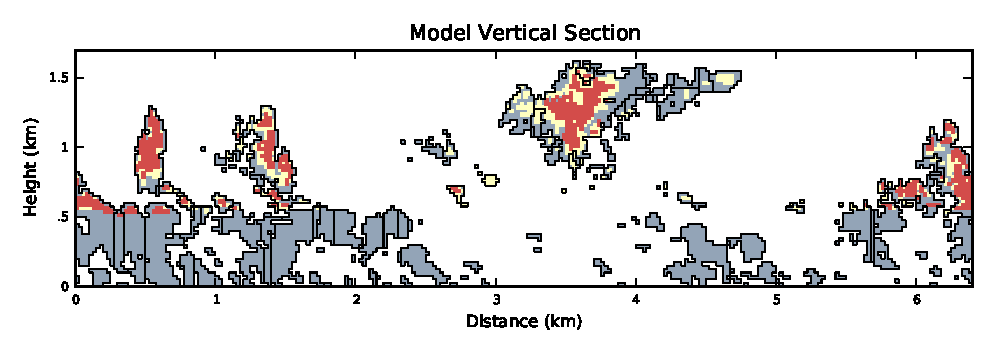
\includegraphics[width=\textwidth]{./figures/vertical_section}
\end{center}
\caption{Vertical section through the BOMEX model, showing the cloud core
(red), the cloud (yellow) and the plume (blue) regions used by the cloud 
tracking algorithm. Black lines show the edges of ``cloudlets" identified by 
the cloud tracking algorithm.}
\label{fig:vertical_section}
\end{figure*}

%f
\begin{figure*}[t]
\vspace*{2mm}
\begin{center}
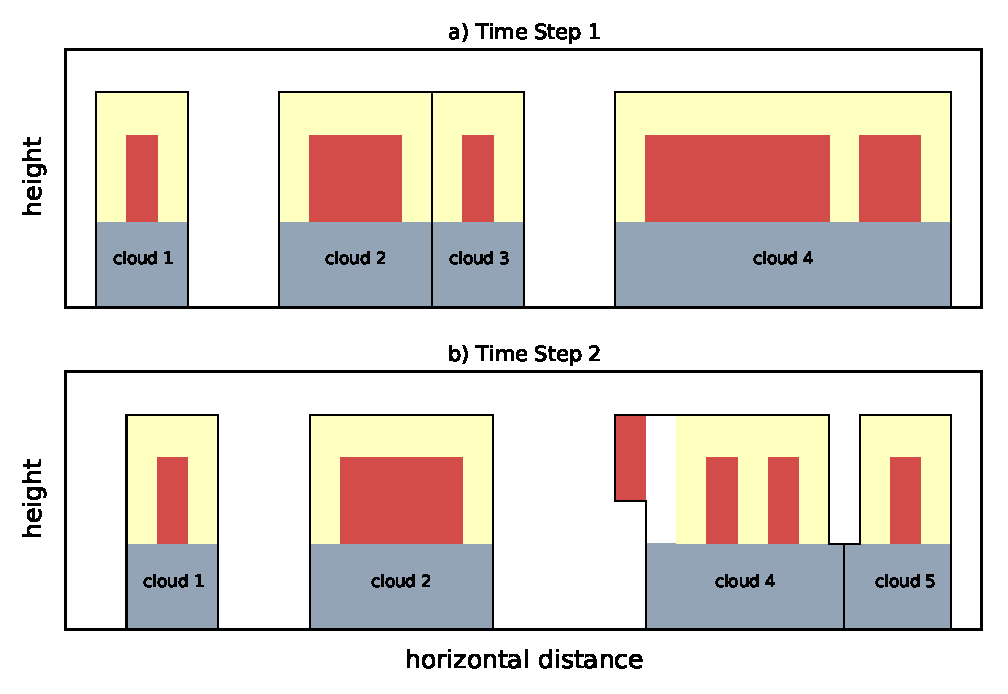
\includegraphics[width=\textwidth]{./figures/cloudfinder_instructions}
\end{center}
\caption{Schematic representation of our cloud tracking algorithm.}
\label{fig:cloudfinder_instructions}
\end{figure*}

%f
\begin{figure*}[t]
\vspace*{2mm}
\begin{center}
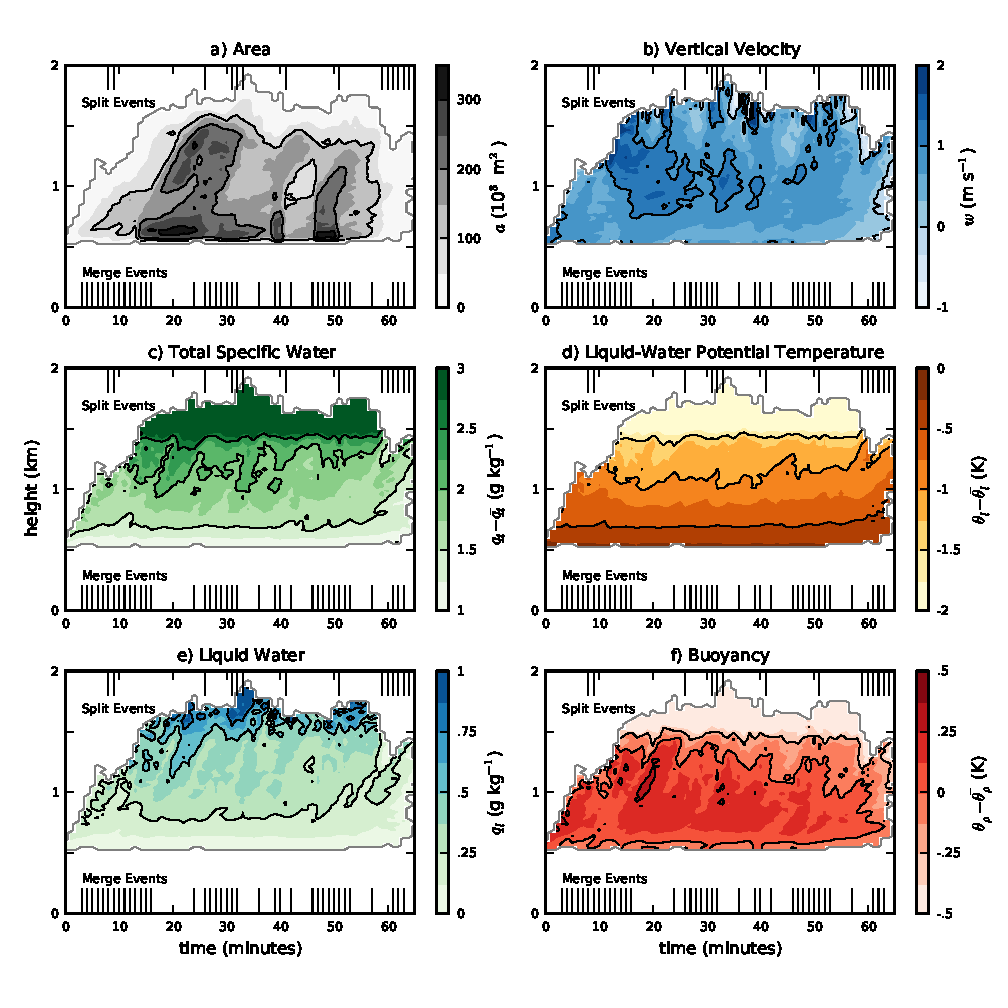
\includegraphics[width=\textwidth]{./figures/example_cloud}
\end{center}
\caption{Height-time profiles of cloud properties of the longest-lived cloud 
in the BOMEX simulation.}
\label{fig:example_cloud}
\end{figure*}

%f
\begin{figure*}[t]
\vspace*{2mm}
\begin{center}
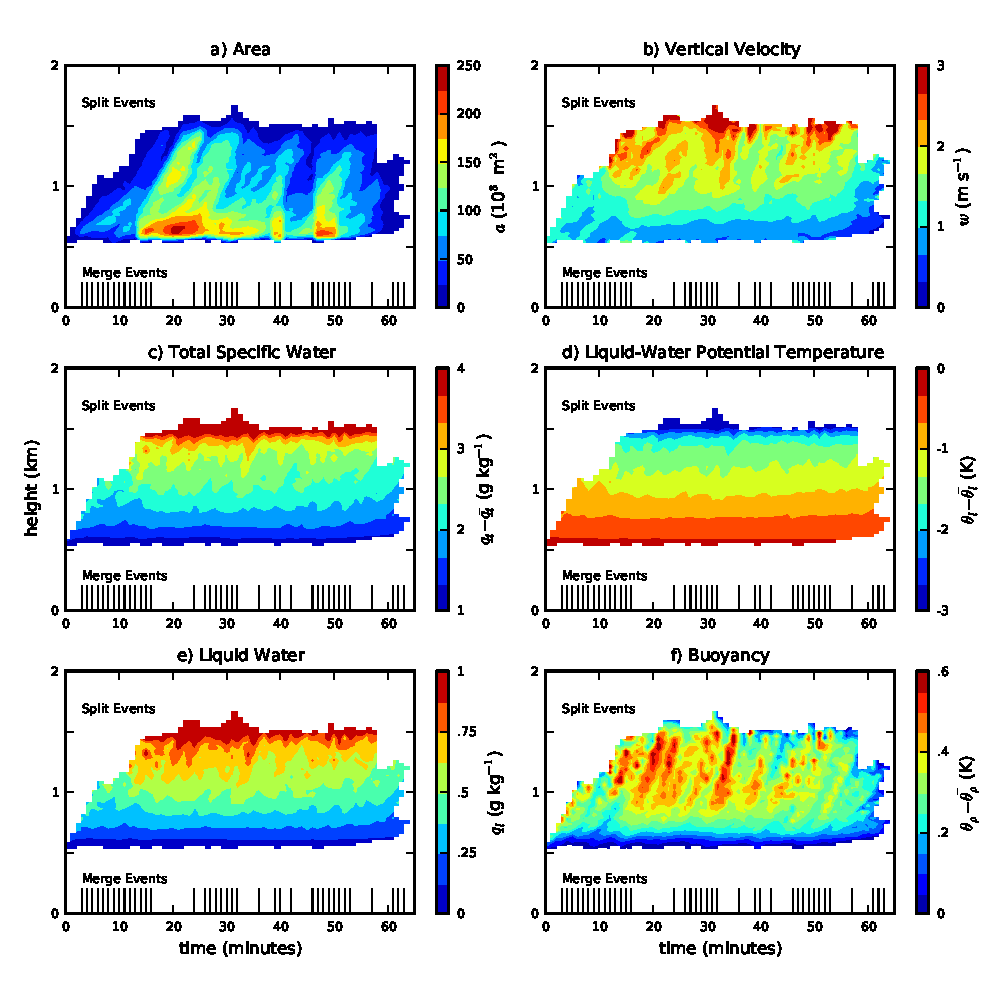
\includegraphics[width=\textwidth]{./figures/example_core}
\end{center}
\caption{Height-time profiles of core properties of the longest-lived cloud in 
the BOMEX simulation.}
\label{fig:example_core}
\end{figure*}

%f
\begin{figure*}[t]
\vspace*{2mm}
\begin{center}
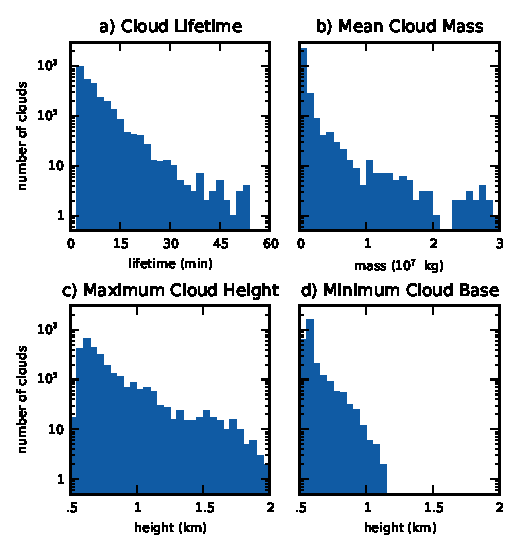
\includegraphics[width=\textwidth]{./figures/cloud_stats}
\end{center}
\caption{Histograms of cloud lifetimes and heights.}
\label{fig:cloud_stats}
\end{figure*}

%f
\begin{figure}[t]
\vspace*{2mm}
\begin{center}
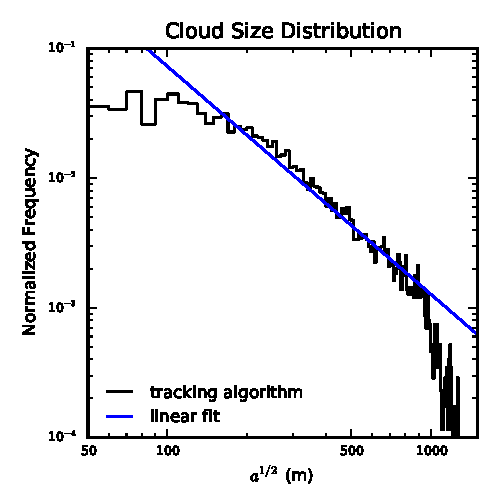
\includegraphics[width=8.3cm]{./figures/cloud_areas}
\end{center}
\caption{Cloud size density}
\label{fig:cloud_areas}
\end{figure}

%f
\begin{figure*}[t]
\vspace*{2mm}
\begin{center}
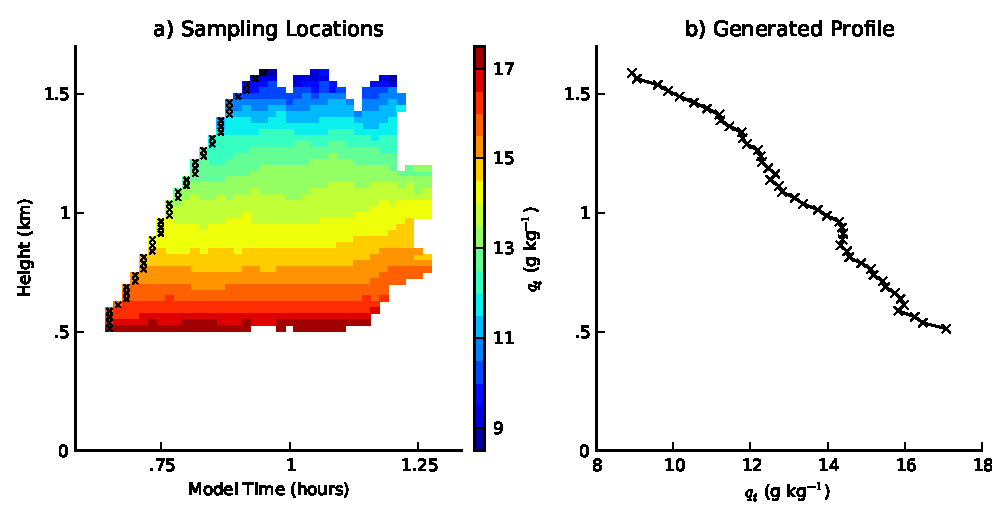
\includegraphics[width=\textwidth]{./figures/cloud_environment_schematic}
\end{center}
\caption{Schematic of encountered cloud environment calculation.}
\label{fig:cloud_environment_schematic}
\end{figure*}

%f
\begin{figure*}[t]
\vspace*{2mm}
\begin{center}
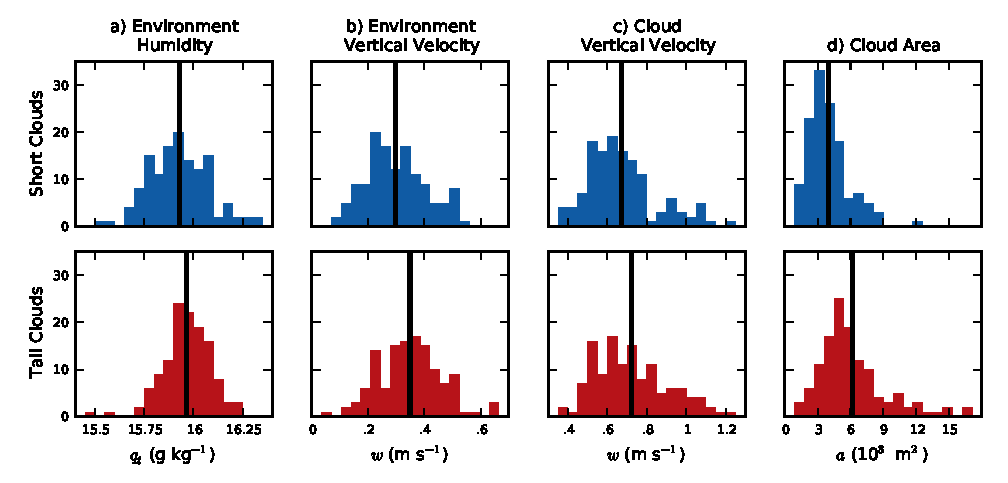
\includegraphics[width=\textwidth]{./figures/cloud_environment_histograms}
\end{center}
\caption{Histograms of encountered cloud environment.}
\label{fig:cloud_envionment_histograms}
\end{figure*}

%f
\begin{figure*}[t]
\vspace*{2mm}
\begin{center}
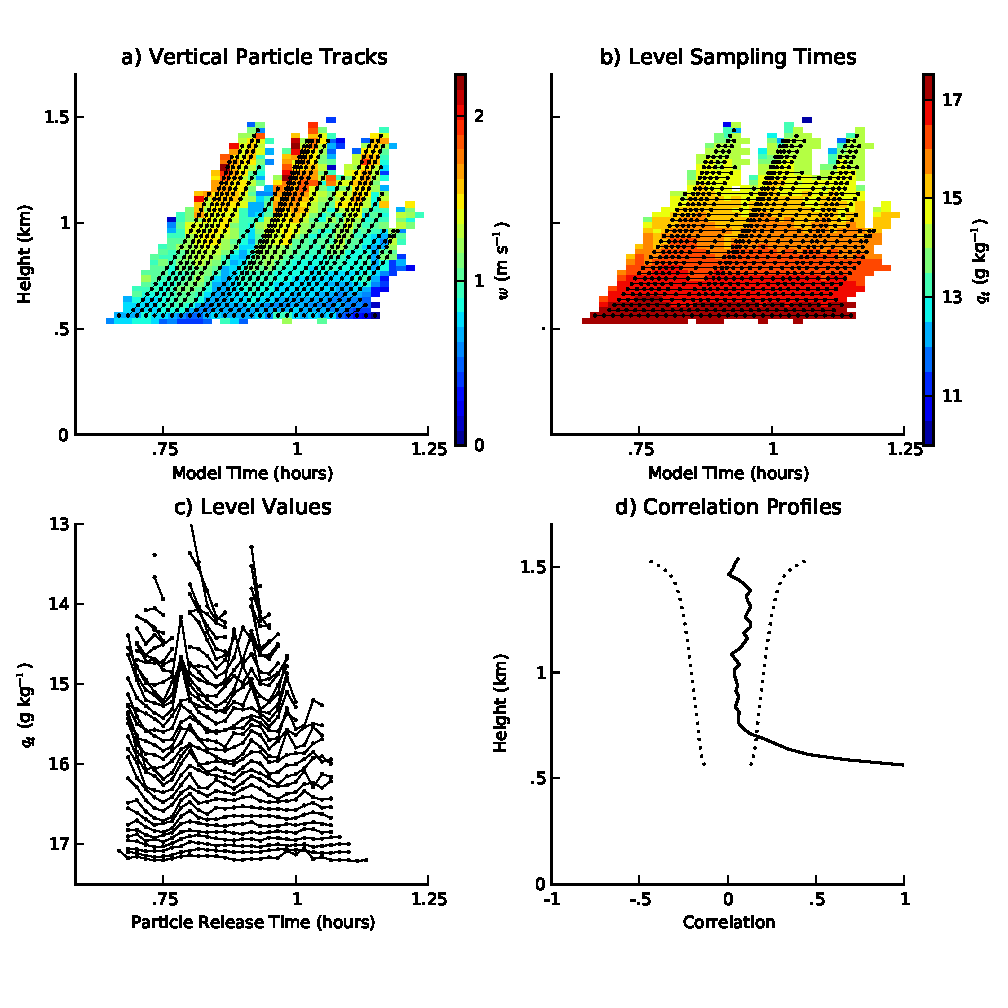
\includegraphics[width=\textwidth]{./figures/cloud_base_schematic}
\end{center}
\caption{Schematic of cloud base correlation calculation.}
\label{fig:cloud_base_schematic}
\end{figure*}

%f
\begin{figure}[t]
\vspace*{2mm}
\begin{center}
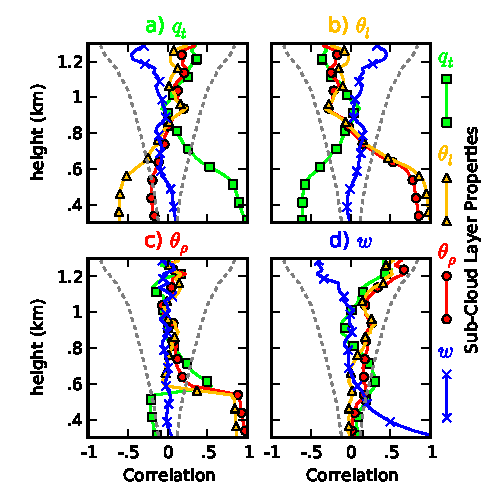
\includegraphics[width=8.3cm]{./figures/sub_cloud_profiles}
\end{center}
\caption{Correlation profiles between sub-cloud properties and various cloud heights.}
\label{fig:sub_cloud_profiles}
\end{figure}

%f
\begin{figure*}[t]
\vspace*{2mm}
\begin{center}
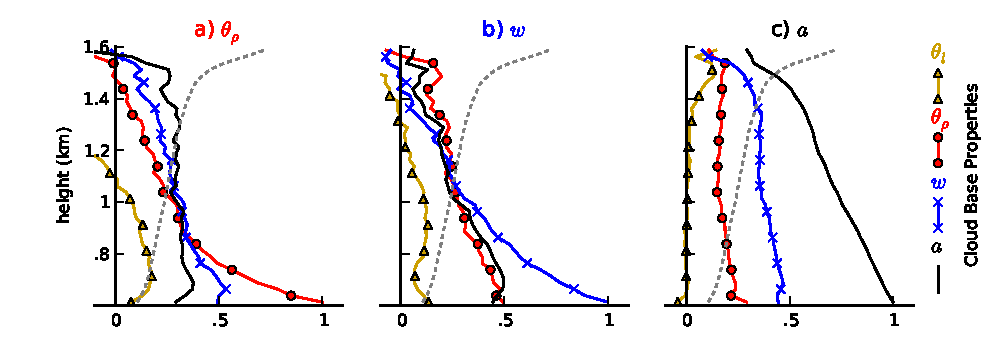
\includegraphics[width=\textwidth]{./figures/cloud_base_profiles}
\end{center}
\caption{Correlation profiles between cloud base and various cloud heights.}
\label{fig:cloud_base_profiles}
\end{figure*}

%f
\begin{figure*}[t]
\vspace*{2mm}
\begin{center}
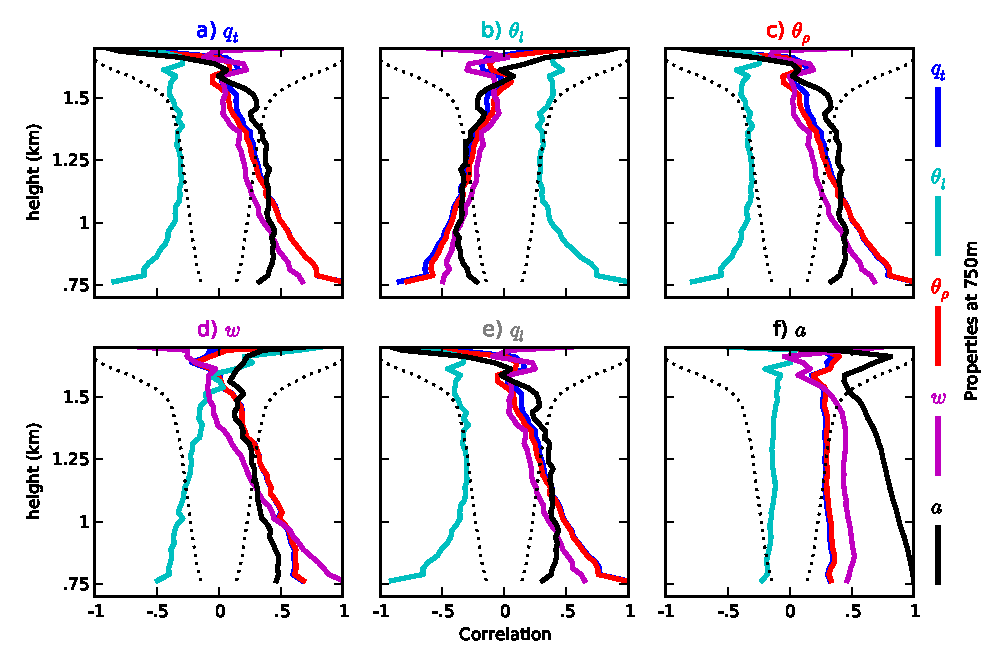
\includegraphics[width=\textwidth]{./figures/750m_profiles}
\end{center}
\caption{Correlation profiles between 750m properties and various cloud heights.}
\label{fig:750m_profiles}
\end{figure*}

%f
\begin{figure}[t]
\vspace*{2mm}
\begin{center}
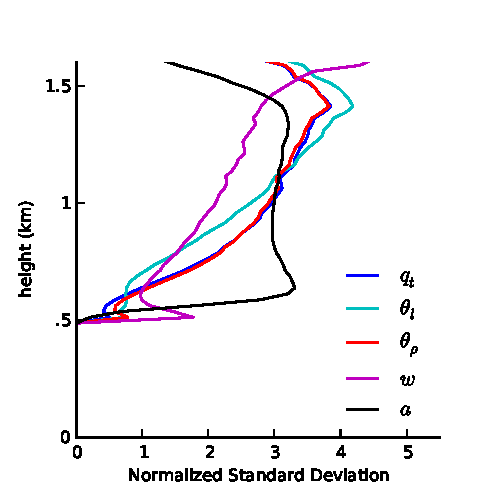
\includegraphics[width=8.3cm]{./figures/st_dev}
\end{center}
\caption{Normalized standard deviations}
\label{fig:st_dev}
\end{figure}

%% TABLES %%%%%%%%%%%%%%%%%%%%%%%%%%%%%%%%%%%%%%%%%%%%%%%%%%%%%%%%%%%%%%%%%%%%


%% ONE-COLUMN TABLE

%t
%\begin{table}[t]
%\label{tbl:cloud_stats}
%\caption{Statistics of tracked clouds}
%\vskip4mm
%\centering
%\begin{tabular}{llcr}
%\tophline
%&&BOMEX\\
%\middlehline
%Total Clouds&&1480\\
%Starts\\
%&Broken&64\\
%&Split&539\\
%&New&877\\
%Ends\\
%&Broken&56\\
%&Merge&91\\
%&Decay&1333\\

%\bottomhline
%\end{tabular}
%\end{table}

%t
%\begin{table}[t]
%\caption{t-test Results}
%\vskip4mm
%\centering
%\begin{tabular}{lcccc}
%\tophline
%&Variable&t-test value&Significance&Direction\\
%\middlehline
%environment&&&\\
%& $q_t$ & -1.33 & 81\% & n/a\\
%& $q_n$ & 0.02 & 2\% & n/a\\
%& tracer & 0.72 & 53\% & n/a\\
%& $\theta_l$ & 2.53 & 98\% & $\downarrow$\\
%& $\theta_v$ & 2.77 & 99.4\% & $\downarrow$\\
%& $w$ & -4.99 & 99.9999\% & $\uparrow$\\
%core&&&\\
%& $q_t$ & 1.57 & 88\% & n/a \\
%& $q_n$ & -0.04 &  3\% & n/a \\
%& $\theta_l$ & -2.10 & 96\% & $\uparrow$ \\
%& $\theta_v$ & -3.55 & 99.96\% & $\uparrow$ \\
% $w$ & -4.21 & 99.997\% & $\uparrow$ \\
%& $\chi_c$ & -5.14 & 99.99995\% & $\uparrow$ \\
%& $a$ & -7.10 & 99.999999992\% & $\uparrow$ \\

%\bottomhline
%\end{tabular}
%\end{table}

%% TWO-COLUMN TABLE

t
\begin{table*}[t]
\label{tbl:mannwhitneyu}
\caption{t-test results}
\vskip4mm
\centering
\begin{tabular}{lccccclr}
\tophline
& Variable & N tall & N small & $\Delta$ mean & $\Delta$ mean/st. dev. & U value & p value\\
\middlehline
environment 550-750 m & & 131 & 136 & & & & \\
& $q_t$       & & &  0.03 g kg$^{-1}$          &  0.24 & 6803   & 0.015    \\ 
& $\theta_l$ & & & -0.008 K                   & -0.19 & 7173.5 & 0.07    \\
& $\theta_\rho$ & & & -0.002 K                   & -0.09 & 7767   & 0.42    \\
& $w$         & & &  0.05 m s$^{-1}$           &  0.45 & 6113   & 3.3x10$^{-4}$ \\
cloud 550-750 m & & & & & & \\
& $q_t$       & & &  0.018 g kg$^{-1}$         &  0.19 & 7358   & 0.13   \\
& $q_l$       & & &  4.9x10$^{-3}$ g kg$^{-1}$ &  0.16 & 7533   & 0.23   \\
& $\theta_l$ & & & -8.6x10$^{-5}$ K           & -0.004 & 8083.5 & 0.78 \\
& $\theta_\rho$ & & &  0.013 K                   &  0.20 & 7350   & 0.13  \\
& $w$         & & &  0.05 m s$^{-1}$           &  0.28 & 6911   & 0.024  \\
& $a$         & & &  2138 m$^2$                &  0.78 & 4282.5 & 2.6x10$^{-11}$ \\
environment 750-1000 m & & 127 & 113 & & & & \\
& $q_t$       & & &  0.03 g kg$^{-1}$          &  0.14 & 6574 & 0.26    \\
& $\theta_l$ & & & -0.007 K                   & -0.12 & 6533 & 0.23    \\
& $\theta_\rho$ & & & -0.003 K                   & -0.08 & 6888 & 0.59    \\
& $w$         & & &  0.05 m s$^{-1}$           &  0.45 & 5145 & 1.6x10$^{-4}$ \\
cloud 750-1000 m & & & & & &          \\
& $q_t$       & & &  0.1 g kg$^{-1}$           &  0.70 & 4368   & 1.7x10$^{-7}$ \\
& $q_l$       & & &  0.04 g kg$^{-1}$          &  0.66 & 4468   & 4.6x10$^{-7}$ \\
& $\theta_l$ & & & -0.03 K                    & -0.51 & 4974   & 4.1x10$^{-5}$  \\
& $\theta_\rho$ & & &  0.07 K                    &  0.71 & 4290   & 7.7x10$^{-8}$ \\
& $w$         & & &  0.11 m s$^{-1}$           &  0.46 & 5225   & 2.8x10$^{-4}$  \\
& $a$         & & &  2661 m$^2$                &  0.89 & 3333.5 & 8.3x10$^{-13}$ \\

\bottomhline
\end{tabular}
\end{table*}

%% The different columns must be seperated with a & command and should
%% end with \\ to identify the column brake.

%%%%%%%%%%%%%%%%%%%%%%%%%%%%%%%%%%%%%%%%%%%%%%%%%%%%%%%%%%%%%%%%%%%%%%%%%%%%%%


%% If figures and tables must be numbered 1a, 1b, etc. the following command
%% should be inserted before the begin{} command.

%\addtocounter{figure}{-1}\renewcommand{\thefigure}{\arabic{figure}a}


\end{document}
